\section{Introduction}
\label{sec:intro}
Virtual memory management lies at the core of modern OS kernel implementation. It is deeply intertwined with most other parts of a typical general-purpose OS kernel design, including scheduling, hardware drivers, and even the filesystem buffer cache. In writing the authoritative reference on the internals of the Solaris kernel, McDougall and Mauro went so far as to claim that ``\emph{the virtual memory sub-system can be considered the core of a Solaris instance, and the implementation of Solaris virtual memory affects just about every other subsystem in the operating system}''~\cite{mcdougall2006solaris}.
This makes rich support for verification the virtual memory management subsystem of an OS kernel critical to the correctness of every other piece of an OS or any software running atop it.

At its core, the virtual memory functionality of modern CPUs is about \emph{location virtualization}: the memory locations
(addresses) seen by most code are not, in fact, the exact location in physical memory where data reside. Instead these 
are \emph{virtual} addresses, which are mapped to actual physical resources by the cooperation of the hardware and OS. 
This is what enables separation of process memory resources:
the OS manipulates hardware functionality to ensure that any attempt by a process to access memory not explicitly granted 
to it by the kernel will fail. But this is complicated by the fact that 
%the OS and hardware can also enable, shared (overlapping) access to physical memory regions; the fact that the kernel data structures themselves are accessed via virtual memory addresses; 
%and the fact that 
control over these mappings of virtual to physical addresses is itself mediated by \emph{in-memory data structures}, 
which the kernel still accesses via virtual address, leading to indirect cycles.

Further complicating matters is that addresses themselves bear no information about which address space they originate 
from. For user processes this is of little concern, as these have access to only their own address space. But the kernel has
(or can grant itself) access to all address spaces. Mixing up addresses from different address spaces leads to severe bugs.
More concerning, keeping track of which \emph{assertions} hold in different address spaces during kernel verification is 
difficult: some assertions should hold across all address spaces, while others hold in only one, and others may hold in 
multiple but still not all.

This kind of context-dependent assertion, where a fact may be true in one address space but not others, has a modal flavor. 
We propose tackling the verification of virtual memory subsystems (and kernels more broadly) by adapting ideas from hybrid
modal logic, which can label assertions true under \emph{other, named} circumstances (i.e., in another address space) with a 
modality indexed by a name for that space (in our case, the root of the page tables for an address space). This offers a 
\textit{convenient} and \textit{powerful} way to \emph{modularly}
\begin{itemize}
\item isolate assertions specific to a particular address space,
\item explicitly state when an assertion is true across address spaces,
\item manipulate address spaces from within other address spaces, and
\item reason about change in address spaces.
\end{itemize}
These advantages make this approach to reasoning about virtual memory more flexible than prior program logic techniques~\cite{kolanski08vstte,kolanski09tphols}, 
which were only able to work with a single address space (the current address space on the CPU) because they were unable
to speak directly \emph{within the logic} about other address spaces.
%\begin{figure}
%   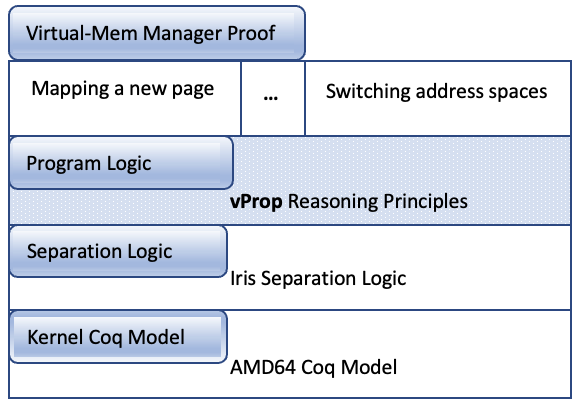
\includegraphics[width=0.5\columnwidth]{architecture.png}
%  \caption{Layers of Implementation}
%  \todo[inline]{Colin says: I don't think this figure helps readers; it is too abstract}
%  \label{fig:architecture}
%\end{figure}

\begin{itemize}
\item We develop these ideas in the form of a logic for working with virtual-address-space-relative assertions,
      implemented as an embedded separation logic within Iris~\cite{jung2018iris} separation logic.
\item We prove the soundness of our \textsf{vProp} logic with respect to a RISC-like fragment of \textsf{AMD64} instructions.
\item We verify simplified versions of several critical virtual-memory-related pieces of OS functionality, 
      including mapping  pages, and the assembly code for switching address spaces. 
      The latter in particular goes beyond the capabilities of prior work, and reveals unexpected
	subtleties.
\end{itemize}
